\chapter{Trabajo relacionado y Estado del Arte} \label{chp:state-of-the-art}

% Relacionar con lo hablado en Introducción
En esta sección se trata y expone el estado actual de las tecnologías utilizadas en 
este proyecto, así como la presentación de proyectos previos y similares a este,
proporcionando una visión necesaria para la comprensión del trabajo realizado.


%%%%%%%%%%%%%%%%%%%%%%%%%%%%%%%%%%%%%%%%%%%%%%%%%%%%%%%%%%%%%%%%%%%%%%%%%%%%%%%%
%%%%%%%%%%%%%%%%%%%%%%%%%%%%%%%%%%%%%%%%%%%%%%%%%%%%%%%%%%%%%%%%%%%%%%%%%%%%%%%%


\section{Sistemas publicador/subscriptor basados en contenido} \label{sct:art_sistpubsubcont}

\subsection{Sistemas publicador/subscriptor} \label{ssct:art_sistpubsubcont_sistpubsub}

Los sistemas publicador/subscriptor siguen el paradigma de publicador/subscriptor, siendo los
intermediarios entre los subscriptores (usuarios con interés en recibir cierta información) y 
los publicadores (los productores de dicha información)\cite{paper:padres}.

Su papel consiste en almacenar las subscripciones de los usuarios, y por cada publicación 
recibida, generar una lista de subscriptores interesados en esta y enviar dicha publicación
a cada subscriptor de la lista. Este proceso de verificar que los intereses de un usuario 
(por medio de su subscripción) concuerdan con los parámetros de la publicación se denomina
''machear una publicación con una subscripción'' (o, en su defecto, con las subscripciones
del sistema).

Este paradigma ha permitido la distribución de las publicaciones de forma más eficiente ya
que los usuarios solo reciben la información que desean, y los publicadores no tienen que manejar
las subscripciones de dichos usuarios. 

Esto se conoce como desacoplamiento entre subscriptores y publicadores, que se
puede descomponer en las siguientes dimensiones\cite{}:
\begin{itemize}

    \item Desacoplamiento espacial: los subscriptores no tienen que conocerse 
    entre si.
    
    \item Desacoplamiento temporal: los subscriptores no tienen que participar
    en el sistema de forma simultánea.

    \item Desacoplamiento de la sincronización: los subscriptores no tienen que estar 
    activos en el sistema para recibir las 
    notificaciones\footnote{Publicación que se ha enviado a un usuario al machear con su 
    subscripción\cite{paper:themanyfacesofpubsub}}.
    
\end{itemize}

Los sistemas publicador/subscriptor presentan diferentes variantes, principalmente, en base
al patrón usado para publicaciones y subscripciones\cite{tfm:victor2017}:
\begin{itemize}
    
    \item Basados en tema: Las publicaciones se clasifican mediante una palabra
    clave que identifica el tema de la publicación. Los subscriptores especifican
    esta palabra clave en las subscripciones, de forma que reciban solo las
    notificaciones cuyo tema sea el especificado.
    
    \item Basados en contenido: Las subscripciones especifican los parámetros
    (contenido) de las publicaciones que el usuario quiere recibir.
    
\end{itemize}

A causa de esto, su utilización se ha popularizado en numerosas 
aplicaciones\cite{paper:themanyfacesofpubsub}.

%%%%%%%%%%%%%%%%%%%%%%%%%%%%%%%%%%%%%%%%%%%%%%%%%%%%%%%%%%%%%%%%%%%%%%%%%%%%%%%%

\subsection{SIENA} \label{ssct:art_sistpubsubcont_siena}

SIENA \cite{paper:siena}, cuyo nombre proviene de las iniciales, en inglés, de Scalable Internet 
Event Notification Architectures, es un sistema publicador/subscriptor basado en contenido 
diseñado para maximizar la escalabilidad del sistema. 

Una de las características de SIENA es la introducción de un nuevo tipo de mensaje, los avisos (o
advertisements en inglés). Estos avisos son emitidos por los publicadores previo envío de las 
publicaciones, y sirven para informar al sistema del tipo de eventos que van a producir. 
SIENA también implementa técnicas para analizar las subscripciones que recibe el sistema, de forma
que se minimice la propagación innecesaria de estas por el sistema

A causa de esto, SIENA se ha convertido en el marco de referencia para el diseño e implementación
de sistemas publicador/subscriptor basados en contenido.

%%%%%%%%%%%%%%%%%%%%%%%%%%%%%%%%%%%%%%%%%%%%%%%%%%%%%%%%%%%%%%%%%%%%%%%%%%%%%%%%

\subsection{PADRES} \label{ssct:art_sistpubsubcont_padres}

PADRES\cite{paper:padres} es un sistema publicador/subscriptor basado en contenido cuya arquitectura
se basa en la comunicación punto a punto (\textit{peer-to-peer (P2P)}) entre los usuarios del sistema.

Este sistema implementa algunas características adicionales, como un sistema de reglas de macheo y 
enrutamiento que se aplica a las publicaciones y subscripciones que llegan al sistema, de forma que
se disminuye el tiempo de procesamiento y creación de rutas entre los publicadores/subscriptores y 
el sistema; subscripciones compuestas, las cuales se basan en la representación de una subscripción
por medio de múltiples subscripciones
atómicas\cite{paper:padres}\cite{paper:gryphon}\cite{paper:hermes}.

PADRES ha sido usado en gran variedad de proyectos y casos de uso, debido a su versatilidad y
eficiencia\cite{paper:pubsub_mmo}.


%%%%%%%%%%%%%%%%%%%%%%%%%%%%%%%%%%%%%%%%%%%%%%%%%%%%%%%%%%%%%%%%%%%%%%%%%%%%%%%%

\subsection{E-StreamHub} \label{ssct:art_sistpubsubcont_estreamhub}

% https://oa.upm.es/51464/1/TFM_VICTOR_RAMPEREZ_MARTIN.pdf
% X E-StreamHub
% X StreamHub
% X Cómo funciona E-StreamHub encima de StreamHub
% X Operadores (AP, M, y EP) y desglosar cada uno
% X Manager de E-StreamHub
% X Zookeeper
% X Reglas en la elasticidad y cómo se aplican

E-StreamHub\cite{paper:e-streamhub} es sistema publicador/subscriptor con 
elasticidad\cite{paper:elasticity}, que extiende y mejora un sistema 
publicador/subscriptor escalable llamado StreamHub\cite{paper:streamhub}.

Al estar desarrollado a partir de StreamHub, E-Streamhub utiliza los
operadores definidos en este, que están constituidos por diferentes componentes
(como se puede ver en \autoref{fig:estreamhub-arq}), desplegando 
uno por cada host (o máquina) activo en el sistema, que son:

\textbf{Access Point (AP)}\\
Estos operadores manejan los eventos que recibe el sistema, dividiendo las subscripciones de forma
equitativa entre los \textit{Matchers} activos, mientras que las publicaciones se envían 
mediante broadcast a todos los \textit{Matchers} activos (una copia a cada \textit{Matcher}), lo que
permite comparar las publicaciones con las subscripciones presentes en el sistema de forma
paralela.

\textbf{Matchers (M)}\\
Los \textit{Matchers} se encargan de comparar las publicaciones recibidas con su lista de 
subscripciones, generando una lista de subscripciones cuyos parámetros (intereses) coinciden con los 
de la publicación, que se enviará, junto con la propia publicación, al \textit{Exit Point} 
correspondiente.

\textbf{Exit Point (EP)}\\
Cada \textit{Exit Point} combina las listas de subscripciones generadas por todos los 
\textit{Matchers}, y envía la publicación a cada uno de los subscriptores de la lista final.

\begin{figure}[htpb]
    \centering
    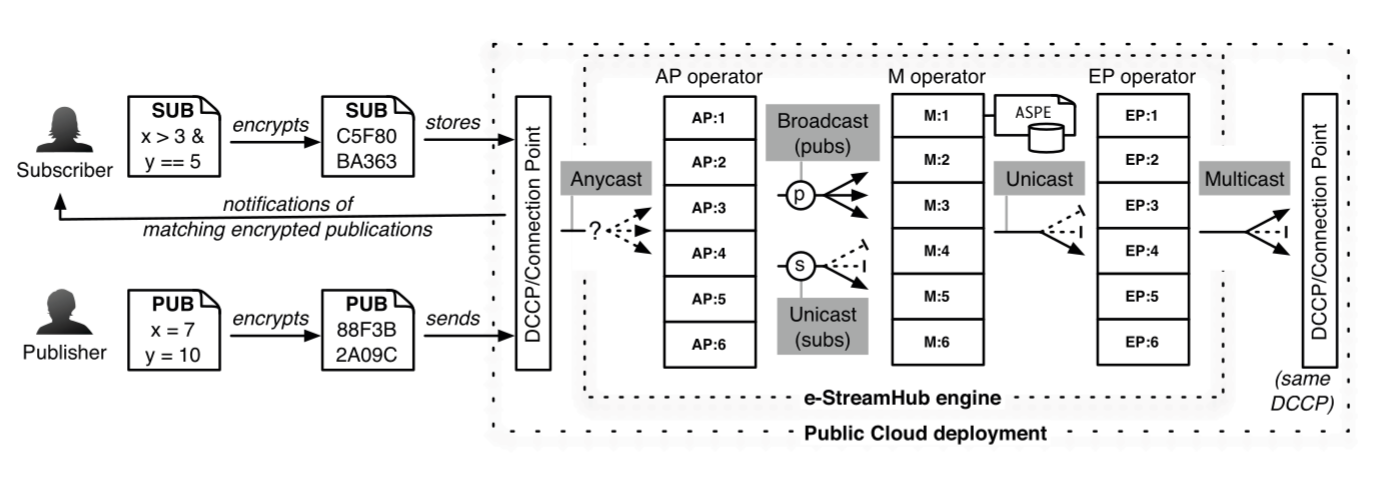
\includegraphics[width=\textwidth]{images/e-strueamhub-arq.png}
    \caption{Ejemplo de un sistema STREAMHUB desplegado en la nube, con 6 instancias de cada operador. Los eventos van de izquierda a derecha. Imagen obtenida de \cite{paper:e-streamhub}.}
    \label{fig:estreamhub-arq}
\end{figure}


La elasticidad de E-StreamHub está implementada mediante la creación de nuevos operadores
en nuevos host cuando estos se necesiten, duplicando los mensajes a procesar en una memoria temporal,
de forma que cuando el nuevo operador esté configurado, pueda comenzar a procesar estos mensajes,
filtrando los obsoletos y minimizando el impacto de esta operación en el sistema.\cite{paper:e-streamhub}

Para poder configurar y manejar los operadores, y las operaciones de creación y eliminación de estos,
E-StreamHub implementa y utiliza un administrador, que monitoriza el estado de los operadores
y lleva a cabo las operaciones de escalado (añadir o eliminar operadores), lo que permite uniformidad
en el sistema y en el manejo de las operaciones de escalado, estableciendo reglas comunes. Al tener
que aplicar una configuración uniforme a todos los operadores, y con el objetivo de poder aplicar esta
configuración y tener control sobre los operadores existentes, E-StreamHub también hace uso
de ZooKeeper\footnote{\href{https://zookeeper.apache.org/}{https://zookeeper.apache.org/}}.

Las reglas a seguir para aplicar las operaciones de escalado se basan en el estado de ciertos recursos
de computación, como el uso de CPU, memoria, etc. Estas reglas, que se aplican para minimizar los
costes a la vez que se maximiza la eficiencia del sistema, se dividen en \textit{locales}, que provocan
que se muevan operadores entre host ya existentes; y \textit{globales}, que hacen que el sistema 
escale, añadiendo o quitando host y moviendo los operadores a otros host con poca carga de trabajo.


%%%%%%%%%%%%%%%%%%%%%%%%%%%%%%%%%%%%%%%%%%%%%%%%%%%%%%%%%%%%%%%%%%%%%%%%%%%%%%%%
%%%%%%%%%%%%%%%%%%%%%%%%%%%%%%%%%%%%%%%%%%%%%%%%%%%%%%%%%%%%%%%%%%%%%%%%%%%%%%%%


\section{Problemas de disponibilidad de cargas de trabajo basadas en contenido} \label{sct:art_sistpubsubcont_problemasdatasetreales}

Uno de los principales problemas actuales en la investigación y desarrollo de sistemas 
publicador/subscriptor es la carencia de cargas de trabajo reales y públicas, que permitan probar los 
sistemas en desarrollo en unas condiciones lo más cercanas a las reales. Estas pruebas son de vital 
importancia para el desarrollo de este tipo de sistemas, ya que ofrecen datos y métricas sobre el
comportamiento final del sistema.

Esta carencia es consecuencia del contenido de los propios datos presentes en las cargas de trabajo,
ya que publicar estas cargas de trabajo puede suponer un problema de seguridad para los usuarios y la
propia empresa que los publica, al contener los intereses (subscripciones) de los
usuarios\cite{paper:lackpublicworkloads}\cite{paper:autoscaling-review}\cite{paper:padres}.


%%%%%%%%%%%%%%%%%%%%%%%%%%%%%%%%%%%%%%%%%%%%%%%%%%%%%%%%%%%%%%%%%%%%%%%%%%%%%%%%
%%%%%%%%%%%%%%%%%%%%%%%%%%%%%%%%%%%%%%%%%%%%%%%%%%%%%%%%%%%%%%%%%%%%%%%%%%%%%%%%


\section{Auto-escalado} \label{sct:art_auto-escaling}

% 0. Contar qué es el auto-escalado
El auto-escalado es la capacidad de un sistema de ajustar (aumentar/disminuir) los recursos computacionales
de os que hace uso de forma automática, en base a la cantidad de trabajo que está recibiendo, y con mínima
o ninguna supervisión humana. Esta característica se ha popularizado en gran medida en los sistemas de
computación en la nube, ya que minimiza los costes en un entorno en el que los recursos son 
\textit{pay-as-you-go}, es decir, solo se paga por los recursos que se usan en cada momento.

Este tipo de sistemas siguen unos requisitos mínimos, especificados en el 
Service Level Agreement o \textit{SLA}, de sus siglas en inglés, el cual es un contrato entre 
el cliente y el propietario de la aplicación. Estos requisitos, por lo general, son las métricas mínimas
del sistema, como por ejemplo, el tiempo de respuesta, el número de mensajes por segundo producidos 
por el sistema (\textit{throughput}\footnote{Para mayor coherencia y brevedad, se usará \textit{throughput} en el resto del documento}).

% 1. Tipos de auto-escalado (especificar el que se va a usar en este trabajo)
El escalado de un sistema puede llevarse a cabo de dos formas diferentes\cite{paper:autoscaling-review}:
\begin{itemize}

    \item[•] \textbf{Escalado horizontal} (\textit{scaling in/out}): añadir o eliminar recursos 
    mediante replicar los ya existentes con el objetivo de balancear el trabajo. Por ejemplo, crear 
    o eliminar una instancia del host para que procese parte del trabajo.

    \item[•] \textbf{Escalado vertical} (\textit{scaling up/down}): añadir o eliminar recursos
    computacionales a un host que ya esté procesando el trabajo recibido. Por ejemplo, aumentar o 
    disminuir la cantidad de CPU dedicada al procesamiento del trabajo recibido.

\end{itemize}

El escalado horizontal es ampliamente usado en los sistemas de computación en la nube, al ofrecer 
mayor flexibilidad a los usuarios en el uso de los recursos 
computacionales\footnote{En este trabajo solo se tratará el escalado horizontal.}. En cambio, el escalado
vertical no se usa en gran medida, ya que, por lo general, los sistemas operativos no permiten cambiar
la cantidad de recursos dedicados a una tarea mientras esta se está llevando a cabo sin reiniciar su 
procesado.

% 2. Mencionar que hay otras clasificaciones de auto-escalables
Adicionalmente, los sistemas auto-escalables se pueden clasificar en reactivos y 
predictivos, es decir, en base a su forma de reaccionar ante una situación que requiera de una 
operación de escalado.

%%%%%%%%%%%%%%%%%%%%%%%%%%%%%%%%%%%%%%%%%%%%%%%%%%%%%%%%%%%%%%%%%%%%%%%%%%%%%%%%

\subsection{Reactivo} \label{ssct:art_auto-escaling_reactive-autoscaling}

Los sistemas auto-escalables que no realizan predicción alguna en la fase de análisis emplean el
\textit{auto-escalado reactivo}, es decir, se limitan a responder al estado actual del sistema,
llevando a cabo las operaciones de escalado requeridas en ese momento, sin tener en cuenta el estado
en el que se podrá encontrar el sistema en el futuro inmediato.

De esta forma, si el sistema se encuentra en una situación en la que la operación de escalado que se 
lleva a cabo no es suficiente para la carga de trabajo que está recibiendo, tendrá que realizar una 
nueva operación de escalado. Este procedimiento puede llevar al sistema, hasta que realice las 
suficientes operaciones de escalado, a proporcionar un servicio por debajo del óptimo y/o esperado.

%%%%%%%%%%%%%%%%%%%%%%%%%%%%%%%%%%%%%%%%%%%%%%%%%%%%%%%%%%%%%%%%%%%%%%%%%%%%%%%%

\subsection{Predictivo} \label{ssct:art_auto-escaling_predictive-autoscaling}

A diferencia del auto-escalado reactivo, el auto-escalado predictivo sí tiene en cuenta el futuro 
inmediato del sistema mediante la aplicación de algoritmos de predicción basados en diferentes métricas,
las cuales pueden basarse, por ejemplo, en el grado de utilización de cierto recurso del sistema en una 
ventana de tiempo previa a la realización de la operación de escalado, en las métricas propias del 
sistema, como tiempos de respuesta, \textit{throughput}, etc.

Este tipo de escalado es capaz de adaptar los recursos disponibles de la forma más óptima del sistema 
a casi cualquier situación en la que aumente la carga de trabajo del sistema, a excepción de los 
incrementos repentinos y sin precedentes, ya que estos son completamente impredecibles.


%%%%%%%%%%%%%%%%%%%%%%%%%%%%%%%%%%%%%%%%%%%%%%%%%%%%%%%%%%%%%%%%%%%%%%%%%%%%%%%%
%%%%%%%%%%%%%%%%%%%%%%%%%%%%%%%%%%%%%%%%%%%%%%%%%%%%%%%%%%%%%%%%%%%%%%%%%%%%%%%%


\section{Cargas de trabajo} \label{sct:art_workloads}

Las cargas de trabajo utilizadas en los sistemas publicador/subscriptor 
representan el número de peticiones de usuarios al sistema, junto con su
tiempo de envío\cite{paper:type_of_workloads}.

Existen 5 tipos de cargas de trabajo en los sistemas de computación en la nube:
\begin{itemize}

    \item \textit{Carga estática}: carga con un número constante de eventos 
    por minuto (ver \autoref{fig:art_workloads-static}).

    \item \textit{Carga creciente}: carga con un rápido incremento en los
    eventos por minuto (ver \autoref{fig:art_workloads-inc}).

    \item \textit{Carga con crecimiento puntual}: carga que presenta un 
    incremento puntual en los eventos por minuto.
    
    \item \textit{Carga periódica}: carga con cambios periódicos en el
    número de eventos por minuto (ver \autoref{fig:art_workloads-periodic}).

    \item \textit{Carga ''On-\&-off''}: carga que presenta periodos en los que
    el número de eventos por minuto es 0 (ver \autoref{fig:art_workloads-periodic}).

    \item \textit{Carga impredecible}: carga que presenta fluctuaciones aleatorias
    en el número de eventos por minuto (ver \autoref{fig:art_workloads-onoff}).

\end{itemize}

En este Trabajo de Fin de Grado, solo se harán uso de las cargas crecientes y 
con crecimiento puntual, al ajustarse a los tipos de pruebas que se desarrollarán, ya 
que estos permitirán, mediante los resultados obtenidos, poder diseñar e implementar
los estudios y/o mejoras necesarias en el auto-escalado del sistema.

\begin{figure}[htpb]
    \centering
    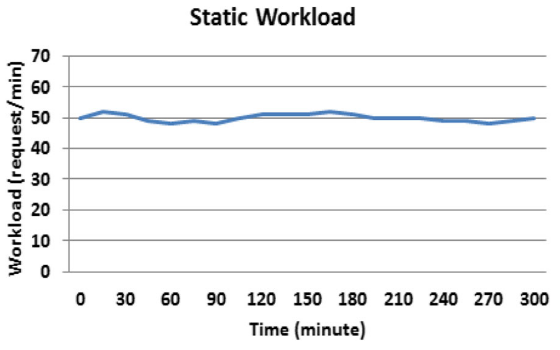
\includegraphics[width=0.5\textwidth]{images/types-of-workload/static-workload.png}
    \caption{\textit{Carga estática.} Imagen obtenida de \cite{paper:type_of_workloads}.}
    \label{fig:art_workloads-static}
\end{figure}

\begin{figure}[htpb]
    \centering
    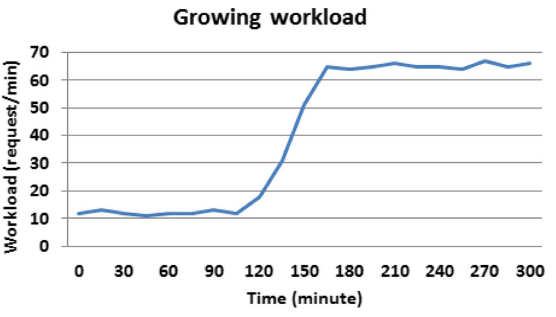
\includegraphics[width=0.5\textwidth]{images/types-of-workload/inc-workload.png}
    \caption{\textit{Carga creciente.} Imagen obtenida de \cite{paper:type_of_workloads}.}
    \label{fig:art_workloads-inc}
\end{figure}

\begin{figure}[htpb]
    \centering
    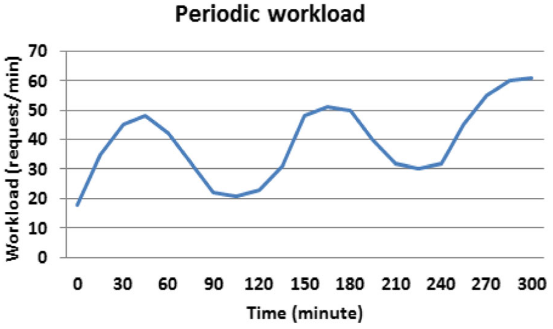
\includegraphics[width=0.5\textwidth]{images/types-of-workload/periodic-workload.png}
    \caption{\textit{Carga periódica.} Imagen obtenida de \cite{paper:type_of_workloads}.}
    \label{fig:art_workloads-periodic}
\end{figure}

\begin{figure}[htpb]
    \centering
    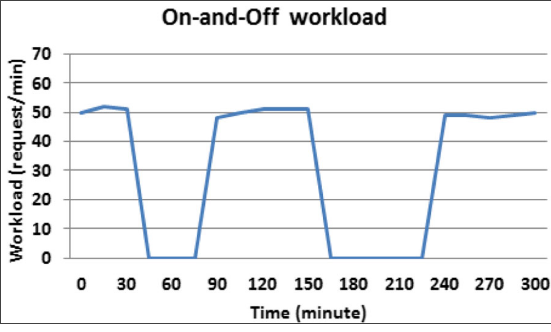
\includegraphics[width=0.5\textwidth]{images/types-of-workload/onoff-workload.png}
    \caption{Carga \textit{''On-\&-off''.} Imagen obtenida de \cite{paper:type_of_workloads}.}
    \label{fig:art_workloads-onoff}
\end{figure}

\begin{figure}[htpb]
    \centering
    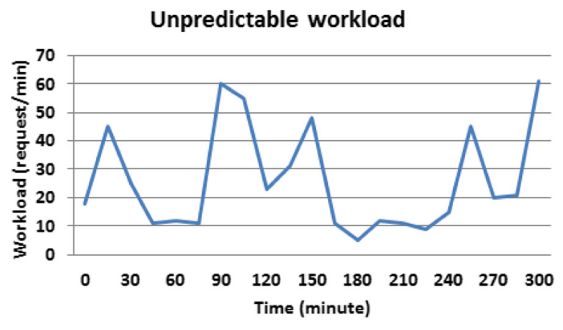
\includegraphics[width=0.5\textwidth]{images/types-of-workload/unpred-workload.png}
    \caption{\textit{Carga inpredecible.} Imagen obtenida de \cite{paper:type_of_workloads}.}
    \label{fig:art_workloads-unpred}
\end{figure}



%%%%%%%%%%%%%%%%%%%%%%%%%%%%%%%%%%%%%%%%%%%%%%%%%%%%%%%%%%%%%%%%%%%%%%%%%%%%%%%%
%%%%%%%%%%%%%%%%%%%%%%%%%%%%%%%%%%%%%%%%%%%%%%%%%%%%%%%%%%%%%%%%%%%%%%%%%%%%%%%%


\section{Estado del Arte} \label{sct:art_stateoftheart}

\subsection{E-SilboPS} \label{ssct:art_stateoftheart_esilbops}

% TFM y Tésis de Victor
% [X] Intro
% [X] Operadores (meter imágen)
% [X] Escalado y algoritmo
% [X] Config (algoritmo ^), comm entre capas (añadir imagen) y Zookeeper

El sistema E-SilboPS, continuación natural del sistema SilboPS y el resultado del 
trabajo de una tesis doctoral\cite{thesis:tesisSVavassori}, es un sistema publicador/subscriptor 
basado en contenido y en contexto, que ha sido diseñado y desarrollado de forma que sea elástico
por defecto.

La arquitectura de este sistema, como se puede comprobar en la \autoref{fig:esilbops-arq} está 
compuesta por cuatro capas de operadores, similar a la encontrada en el sistema 
\textit{StreamHub}\cite{paper:streamhub}, estando cada capa compuesta por una o varias instancias
del correspondiente operador, siendo estos últimos los siguientes:

\textbf{Connection Points (CP)}\\
Estos operadores se encargan de la conexión con los diferentes publicadores y subscriptores y del envío
de las publicaciones correspondientes a los subscriptores interesados en ellas. Los \textit{CP}, que
reciben tanto publicaciones como subscripciones, envían estas a un \textit{Access Point} libre.

\textbf{Access Points (AP)}\\
Los \textit{Access Points}, que reciben publicaciones y subscripciones por igual, se encargan de enviar
la subscripción recibida al \textit{Matcher} seleccionado mediante un selector; mientras que si reciben
una publicación, envían una copia de esta a cada \textit{Matcher}.

\textbf{Matcher (M)}\\
Los \textit{Matchers} almacenan las subscripciones de los usuarios, teniendo cada instancia una pequeña
lista de subscripciones, que serán las que le ha asignado el selector. En cambio, las publicaciones se usan
para comparar los parámetros del contenido deseado por cada subscripción con los de la publicación manejada,
generando una lista de subscriptores interesados en dicha publicación.

\textbf{Exit Points (EP)}\\
Estos operadores, que solo reciben las listas parciales de subscriptores generadas por los \textit{Matchers}
y la publicación correspondiente, componen una lista completa de subscriptores interesados en dicha 
publicación.

\begin{figure}[htpb]
    \centering
    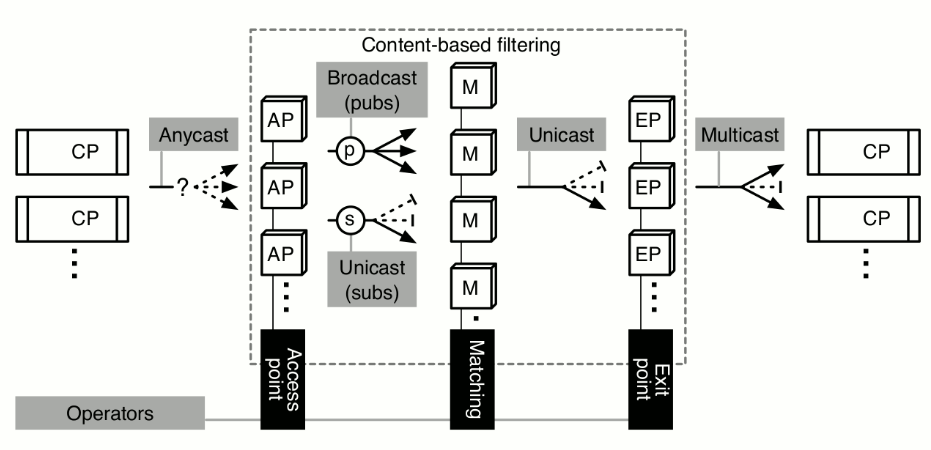
\includegraphics[width=\textwidth]{images/streamhub-arq.png}
    \caption{Arquitectura y funcionamiento de los sistemas \textit{E-SilboPS} y \textit{StreamHub}. Imagen obtenida de \cite{paper:e-streamhub}.}
    \label{fig:esilbops-arq}
\end{figure}

La elasticidad de \textit{E-SilboPS} se basa en la capacidad de cada capa de operadores de añadir o quitar
instancias (operaciones de escalado) de los operadores correspondientes de forma dinámica, ajustando la
capacidad del sistema a los requisitos de este en cada momento, optimizando el uso de los recursos 
computacionales al máximo.

Esta escalabilidad dinámica sin interrumpir el sistema se lleva a cabo gracias al algoritmo de escalado, basado
en el algoritmo de Chandy-Lamport\cite{paper:chandy-lamport}, que permite al sistema seguir operando de
forma normal incluso cuando se está llevando a cabo una operación de escalado.

De forma adicional, y para poder mantener la coordinación y comunicación entre las diferentes capas de 
operadores del sistema, como se observa en la \autoref{fig:esilbops-opcomm} y la consistencia y estabilidad 
del mismo, se requiere del uso de un administrador, que imponga la configuración establecida para cada y su 
coordinación con las demás. El sistema elegido para llevar a cabo esta tarea es
Zookeeper\footnote{\href{https://zookeeper.apache.org/}{https://zookeeper.apache.org/}}.

\begin{figure}[htpb]
    \centering
    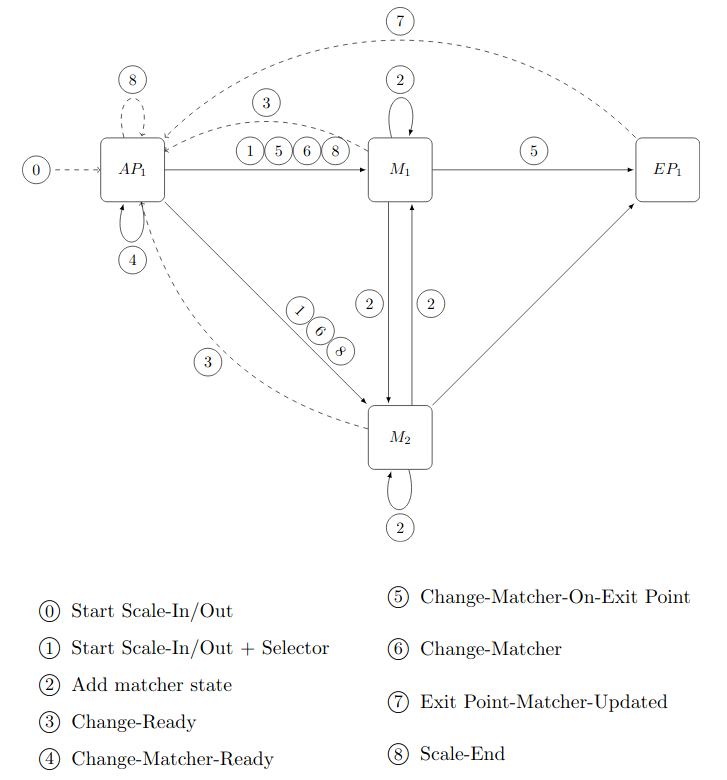
\includegraphics[width=\textwidth]{images/esilbops-opcomm.png}
    \caption{Comunicación y coordinación de las capas de operadores en una operación de escalado de la capa de \textit{Matchers} (M2 es la nueva instancia de \textit{Matcher}). Las lineas continuas representan la comunicación de subscripciones y publicaciones entre capas de operadores, mientras que las discontinuas son mensajes de coordinación para sincronizar las capas y los operadores. Imagen obtenida de \cite{thesis:tesisVictor}.}
    \label{fig:esilbops-opcomm}
\end{figure}

La configuración del sistema y el número de operadores en cada capa se expresa mediante el 
formato \textit{X-Y-Z}, siendo este el número de instancias de los operadores 
\textit{CP}/\textit{AP}, \textit{M} y \textit{EP}, respectivamente.
A lo largo de este documento se usará este formato para expresar la configuración del sistema.


%%%%%%%%%%%%%%%%%%%%%%%%%%%%%%%%%%%%%%%%%%%%%%%%%%%%%%%%%%%%%%%%%%%%%%%%%%%%%%%%
%%%%%%%%%%%%%%%%%%%%%%%%%%%%%%%%%%%%%%%%%%%%%%%%%%%%%%%%%%%%%%%%%%%%%%%%%%%%%%%%


\section{Herramientas utilizadas}

\subsection*{Java}

Java\footnote{\href{https://www.java.com/es/}{https://www.java.com/es/}} es un 
lenguaje de programación orientado a objetos y que sigue un paradigma imperativo.
Ver logo en \autoref{fig:java-logo}.

Tanto E-SilboPS, como los proyectos anteriores se han implementado en Java, por
lo que este trabajo utiliza este lenguaje para desarrollar las pruebas necesarias
para medir el rendimiento del sistema.

\begin{figure}[htpb]
    \centering
    
\includegraphics[width=0.3\linewidth]{images/logos/java-logo.png} 
    \caption{Logo de Java.}
    \label{fig:java-logo}
\end{figure}


\subsection*{R}

R\footnote{\href{https://www.r-project.org/}{https://www.r-project.org/}} es un
lenguaje de programación orientado al análisis estadístico. Ver logo 
en \autoref{fig:r-logo}.

Se ha utilizado R para la realización de las cargas de trabajo, y la generación
de las gráficas incluidas en este TFG, así como la implementación de los modelos
predictivos, debido a la versatilidad y cantidad de herramientas que proporciona
para llevar a cabo estas tareas.

\begin{figure}[htpb]
    \centering
    
\includegraphics[width=0.2\linewidth]{images/logos/R-Logo.png} 
    \caption{Logo de R.}
    \label{fig:r-logo}
\end{figure}


\subsection*{Git}

Git\footnote{\href{https://git-scm.com/}{https://git-scm.com/}} es una herramienta
abierta y de código libre para el control de versiones diseñada para facilitar el
manejo de proyectos, principalmente de código. Ver logo en \autoref{fig:git-logo}.

Para mantener coherencia en el desarrollo y tener un control de versiones del
código, se ha utilizado Git, además de 
GitHub\footnote{\href{https://github.com/}{https://github.com/}} y
GitLab\footnote{\href{https://github.com/}{https://github.com/}}, herramientas web
necesarias para facilitar el manejo y gestión de las diferentes ramas y de los
cambios realizados.


\begin{figure}[htpb]
    \centering
    
\includegraphics[width=0.3\linewidth]{images/logos/git-logo.png} 
    \caption{Logo de Git.}
    \label{fig:git-logo}
\end{figure}


\subsection*{Apache Maven}

Maven\footnote{\href{https://maven.apache.org/index.html}{https://maven.apache.org/index.html}}
es una herramienta para el gestión y creación de proyectos Java, ofreciendo un modelo
de configuración muy accesible y sencillo de manejar para el desarrollador. 
Ver logo en \autoref{fig:maven-logo}.

Se ha utilizado Apache Maven debido a su uso previo en este proyecto, así como la
facilidad que proporciona a los desarrolladores para gestionar proyectos Java.

\begin{figure}[htpb]
    \centering
    
\includegraphics[width=0.3\linewidth]{images/logos/maven-logo.png} 
    \caption{Logo de Apache Maven.}
    \label{fig:maven-logo}
\end{figure}


\subsection*{JUnit 5}

JUnit 5\footnote{\href{https://junit.org/junit5/}{https://junit.org/junit5/}} es un
framework para el desarrollo de pruebas para aplicaciones Java que ha sido ampliamente
usado. Ver logo en \autoref{fig:junit5-logo}.

Para implementar las pruebas del generador de cargas de trabajo reales, así como
las pruebas propias el sistema E-SilboPS, se han usado pruebas de JUnit 5.
Este framework permite validar de forma muy completa el funcionamiento de una
aplicación Java, pudiendo probar y confirmar que el comportamiento y las funciones
de un sistema son las esperadas.

\begin{figure}[htpb]
    \centering
    
\includegraphics[width=0.3\linewidth]{images/logos/junit5-logo.png} 
    \caption{Logo de JUnit 5.}
    \label{fig:junit5-logo}
\end{figure}


%%%%%%%%%%%%%%%%%%%%%%%%%%%%%%%%%%%%%%%%%%%%%%%%%%%%%%%%%%%%%%%%%%%%%%%%%%%%%%%%
%%%%%%%%%%%%%%%%%%%%%%%%%%%%%%%%%%%%%%%%%%%%%%%%%%%%%%%%%%%%%%%%%%%%%%%%%%%%%%%%